\chapter{Premenstrual Syndrome}
\label{applications-priors_knots_select}

A reoccurring theme in the GBD 2010 study is epidemiological data without clear age-patterns.  Unclear age-patterns makes expert priors essential to complement sparse and noisy data in the modeling process.  However, such cases are very sensitive to the choice of prior assumptions, as show in the following example of premenstrual syndrome (PMS) in Western Europe.

PMS is a common cyclic disorder that affects women of reproductive years during the period between ovulation and the onset of menses.  More than 200 behavioral, psychologic and physical symptoms have been associated with PMS, the most common being irritability, tension, depression, bloating, weight gain and food cravings.  There is no known cause or consistent treatment \cite{dickerson_premenstrual_2003, singh_incidence_1998, goodale_alleviation_1990}.

A meta-analysis of data from a systematic review on the descriptive epidemiology of premenstrual syndrome yielded 74 rows of prevalence data, 18 being from Western Europe.  As seen from figure \ref{fig:app-pms_data}, the data is noisy, with overlapping and heterogeneous age groups that show no clear age pattern.

    \begin{figure}[h]
        \begin{center}
            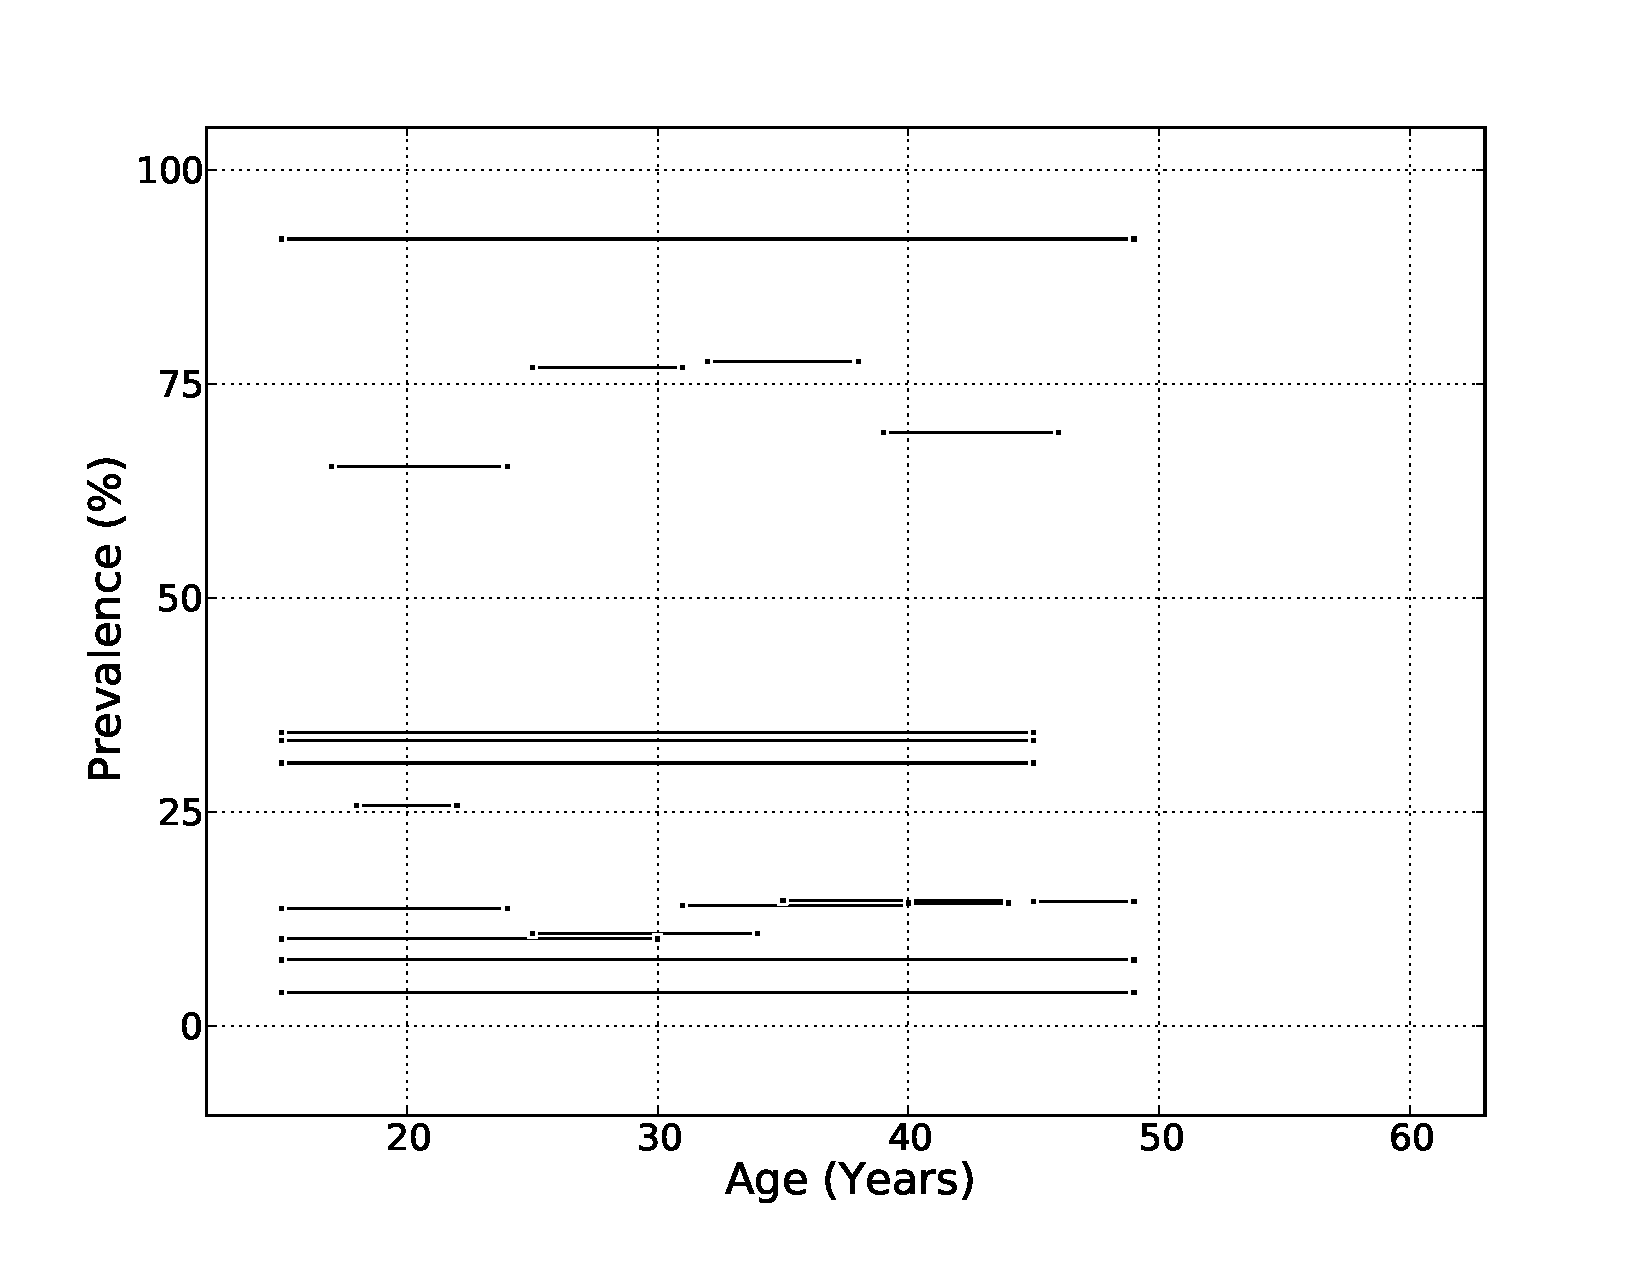
\includegraphics[width=\textwidth]{pms-data.pdf}
            \caption{Prevalence data for women with premenstrual syndrome in Western Europe.}
        \end{center}
        \label{fig:app-pms_data}
    \end{figure}

\section{Priors on level} \label{sec:app-priors on level}
With no clear guidance from the data, informative priors to identify an age pattern are a critical part of the modeling process, even though they may have unintended effects as discussed in Chapter \ref{theory-age_pattern_model}.  To illustrate the effects of priors, an age-standardized negative-binomial mixed effects spline model is used without invoking the compartmental model from Chapter \ref{sys-dynamics}.

Looking at the data in figure \ref{fig:app-pms_data}, no data exists before age 15 or after age 50.  Since PMS is a disorder related to the cycles of the female reproductive system, it is obvious that the data is not present for biological reasons.  However, this information is unknown to the model and with no prior limiting the age range to 15-60, the spline model estimates prevalence for the entire age range of 0-100, as seen in figure \ref{fig:app-prios_on_level}.  Here expert knowledge needs to inform the model that prevalence should not be expected outside of the ages 15-50.

    \begin{figure}
        \begin{center}
            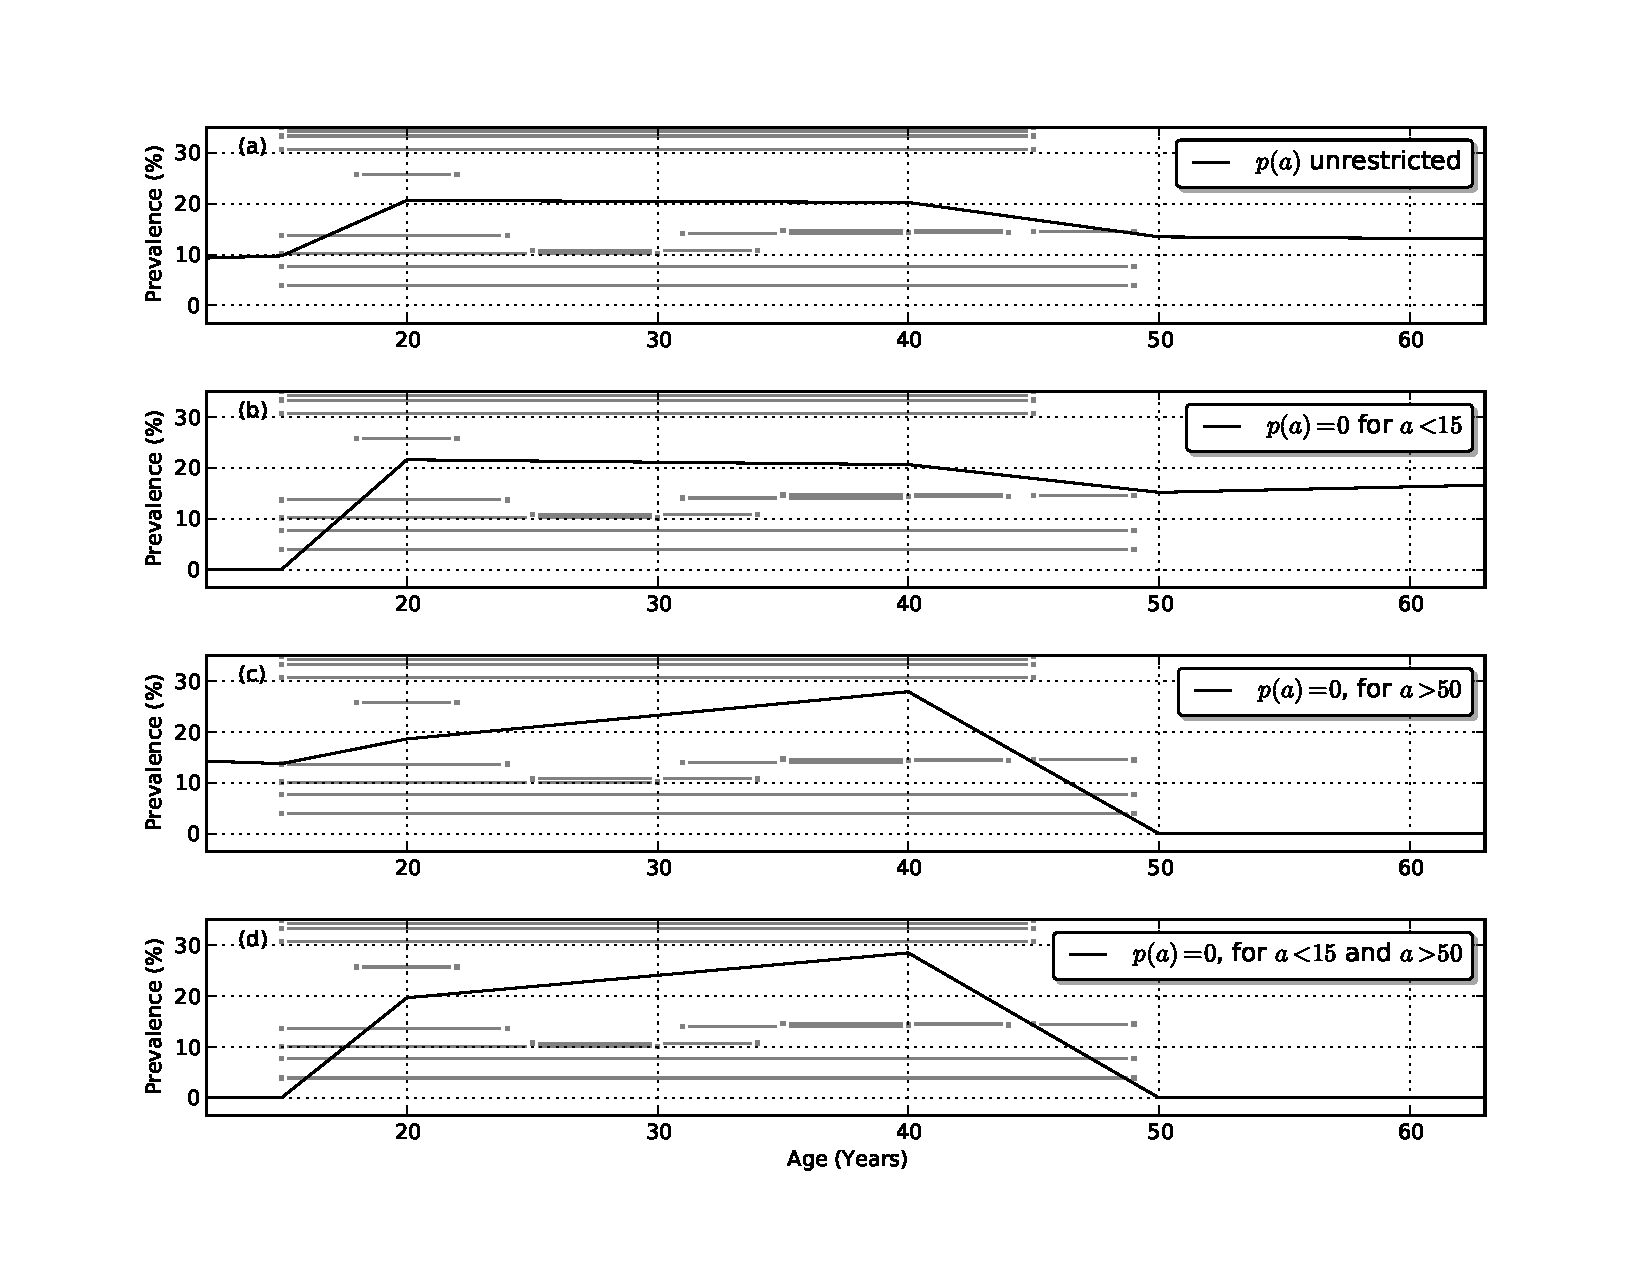
\includegraphics[width=\textwidth]{pms-priors.pdf}
        \end{center}
        \caption{PMS is a disorder related to the cycles of the female reproductive system.  As shown in panel (a), without a level prior to inform the model that prevalence data is not present outside of the ages 15-50 for biological reasons, it will create prevalence estimates for all ages, regardless of biological feasibility.  Restricting prevalence to above age 15 in panel (b), below age 50 in panel (c), or between ages 15-50 in panel (d) changes the prevalence estimates dramatically for women in Western Europe with PMS.}
        \label{fig:app-prios_on_level}
    \end{figure}

\section{Knot location}
As previously discussed in Chapters \ref{theory-age_group_model-overlapping_data} and \ref{applications-splines_knot_loc}, age-specific hazards are modeled with splines, using knots to partition the age range into intervals.  Models will not be very sensitive to choice of knots with ample data and clear age patterns.  However, with sparse and noisy data without a clear age pattern, the number and location of knots can influence the model results substantially as seen in figure \ref{fig:app-knot_loc}.  Choosing the number and location of knots a priori using expert knowledge allows the user to determine critical features of the model.

    \begin{figure}
        \begin{center}
            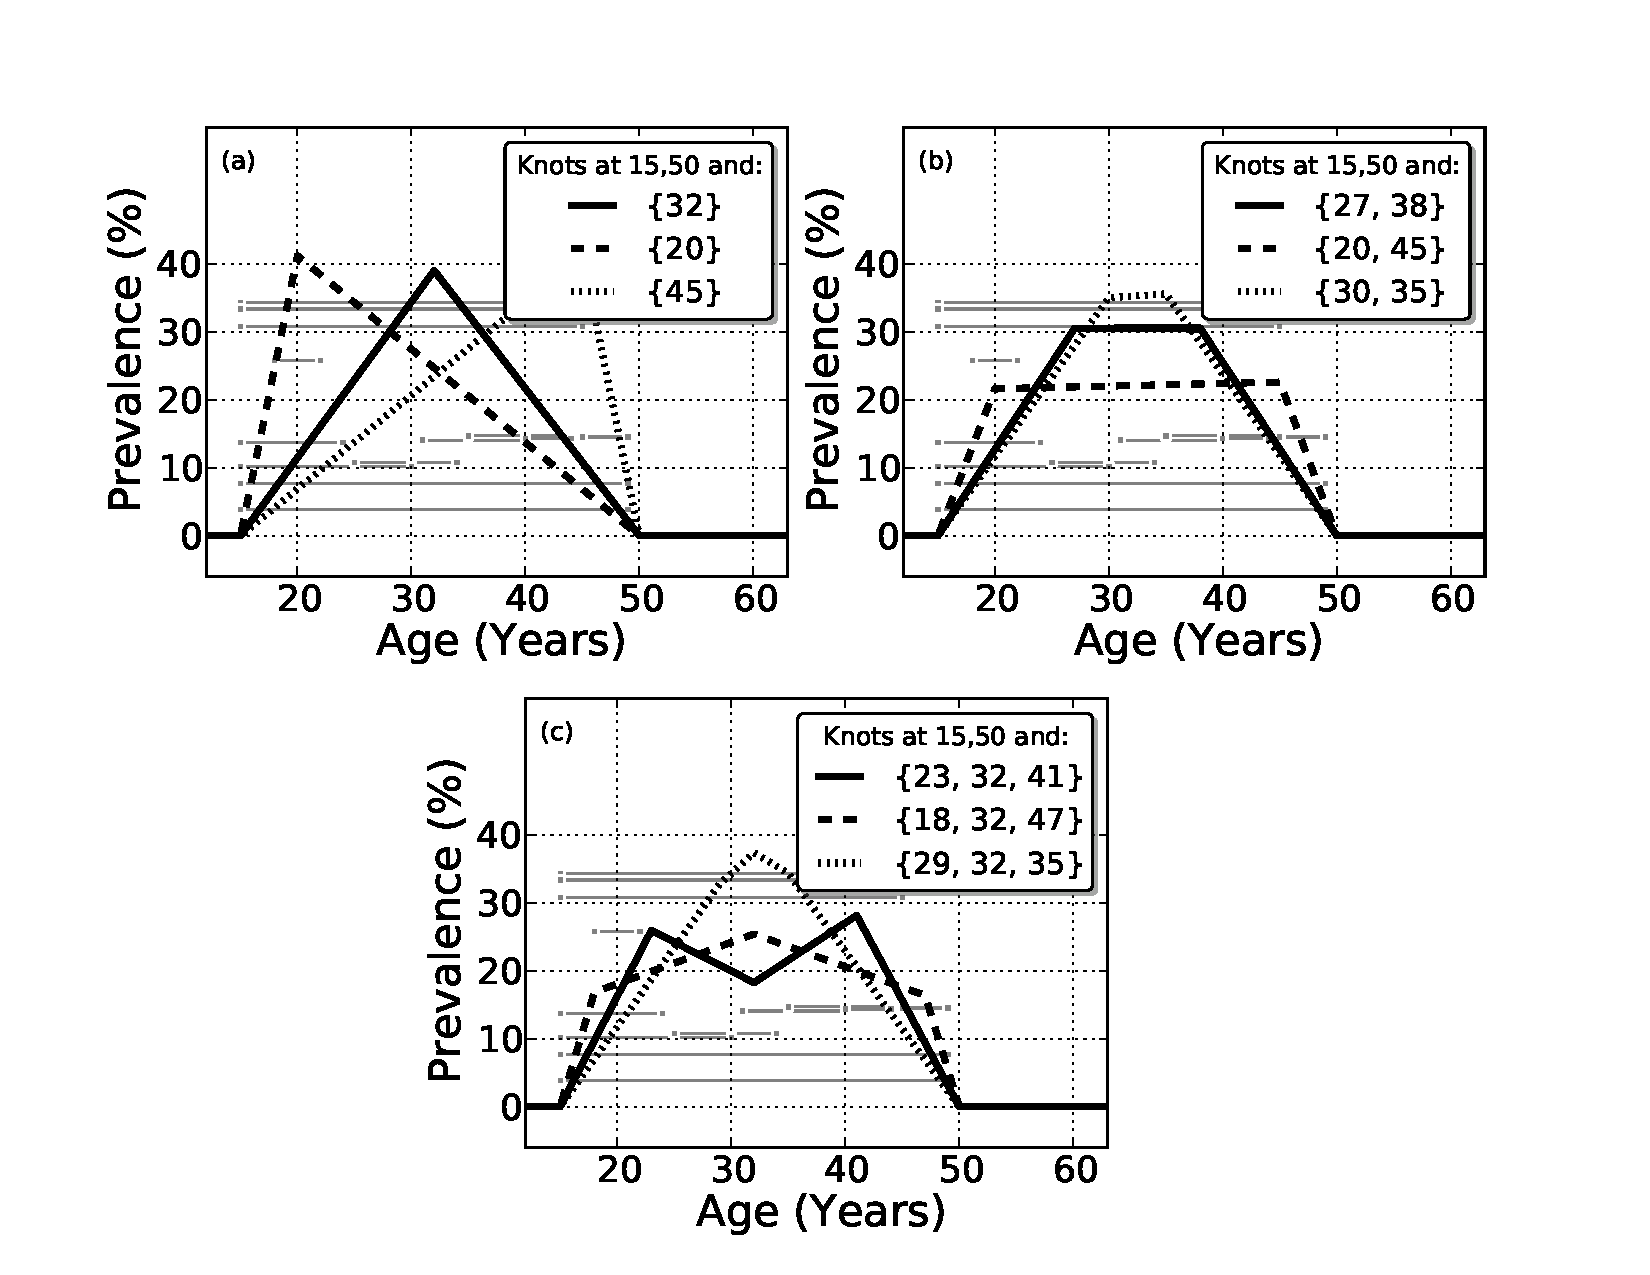
\includegraphics[width=\textwidth]{pms-knot_location.pdf}
        \end{center}
        \caption{All panels have knots at \{0, 15, 50, 100\} and vary the number and location of knots between the ages of 15 and 50 to show the sensitivity of knot selection sparse and noisy data without a clear age pattern. Even with 1 knot, the placement at age 20, 32 or 45 gives markedly different estimates of PMS prevalence in Western Europe (panel (a)).  Panel (b) uses 2 knots and varies their locations at \{27, 38\}, \{20, 45\}, or \{30, 35\} while panel (c) uses 3 knots at locations \{23, 32, 41\}, \{18, 32, 47\} and \{29, 32, 35\}.}
        \label{fig:app-knot_loc}
    \end{figure}

\section{Priors on monotonicity}
Another common prior for age patterns is the belief that the epidemiologic parameter increases or decreases over a certain age range.  As seen in figure \ref{fig:app-knot_loc}, priors on monotonicity between the critical ages of 25 and 40 have a drastic effect on the prevalence estimate for Western Europe.

    \begin{figure}
        \begin{center}
            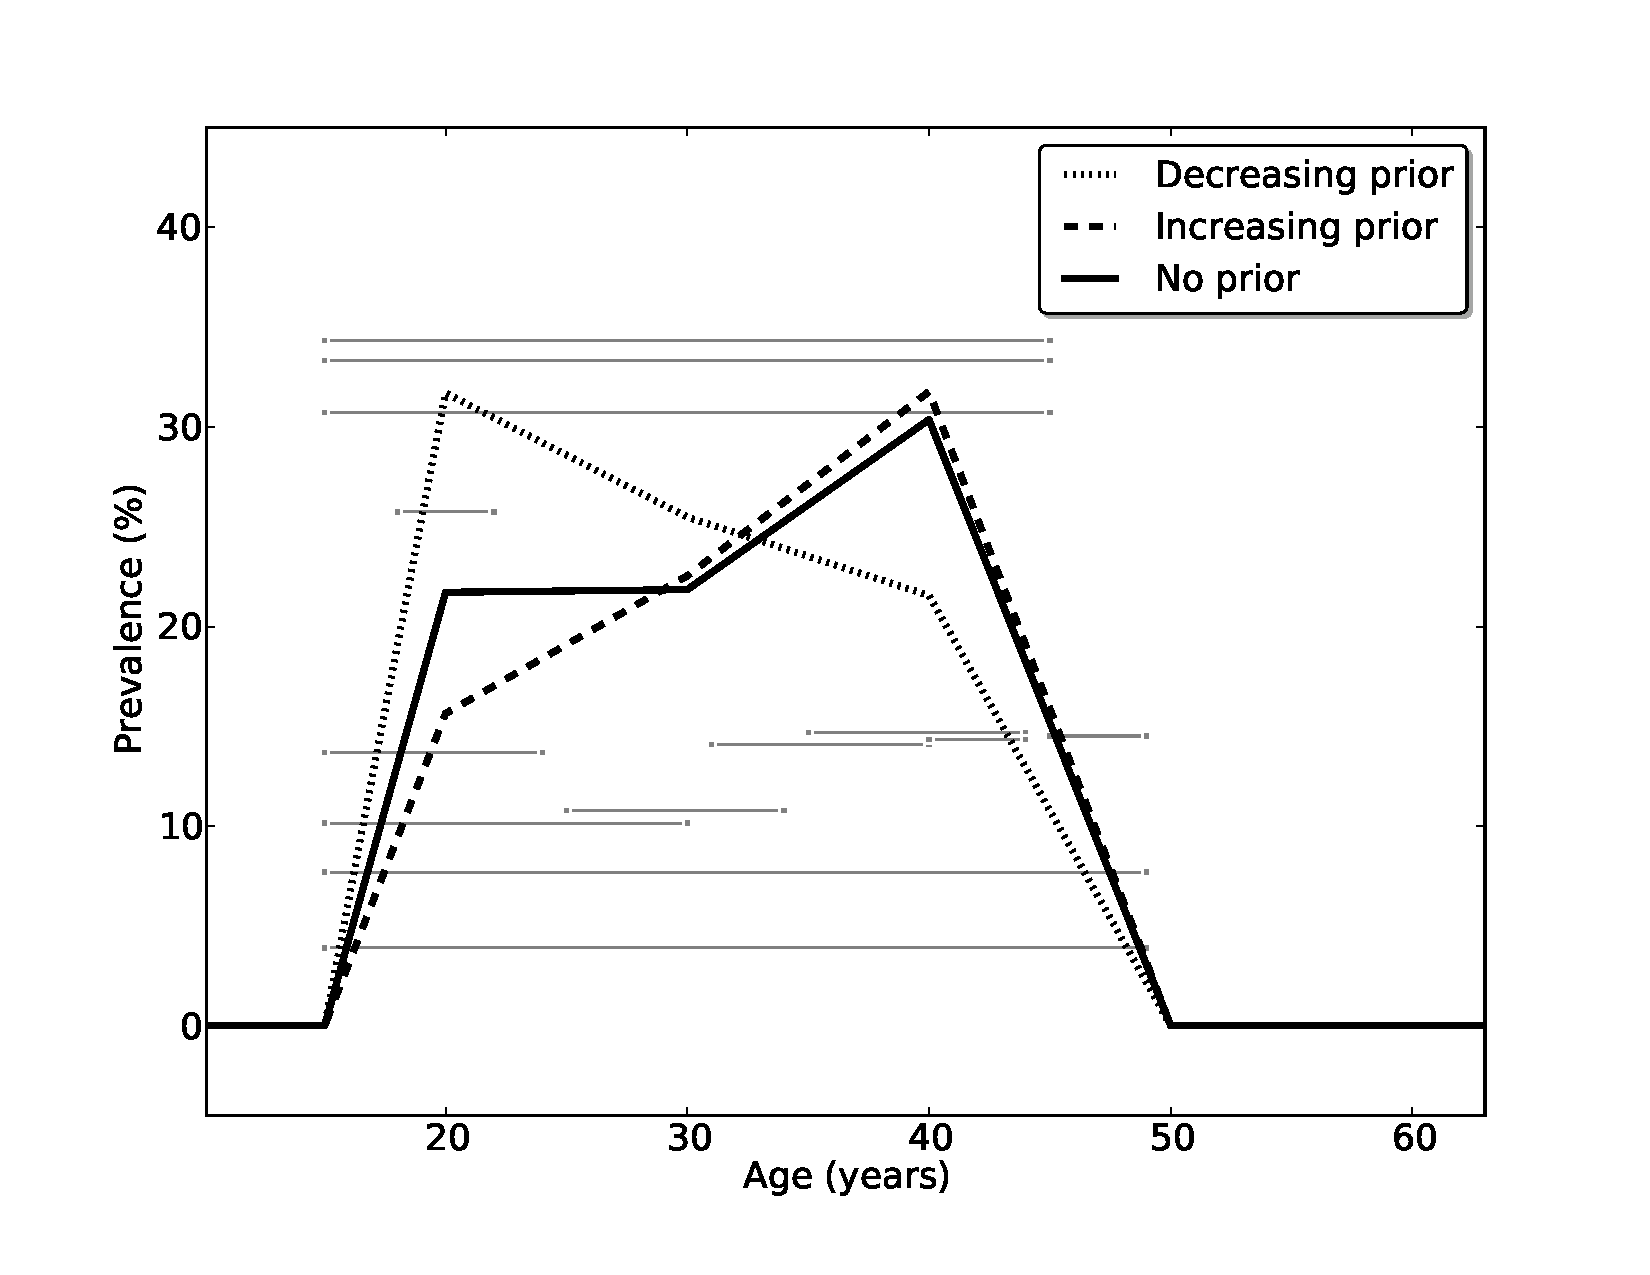
\includegraphics[width=\textwidth]{pms-direction.pdf}
        \end{center}
        \caption{Between the ages of 25-40, the prior on monotonicity makes a large impact on the prevalence estimates for women in Western Europe with premenstrual syndrome.}
        \label{fig:app-knot_loc}
    \end{figure} 